\chapter{Architectural Design}
\label{ch:architectural-design}%

\section{Overview}
\label{sec:overview}%

\par The following is an overview of the S\&C architecture general components. A more detailed view will be provided in
\ref{sec:deployment-view}.

\begin{figure}[H]
      \centering
      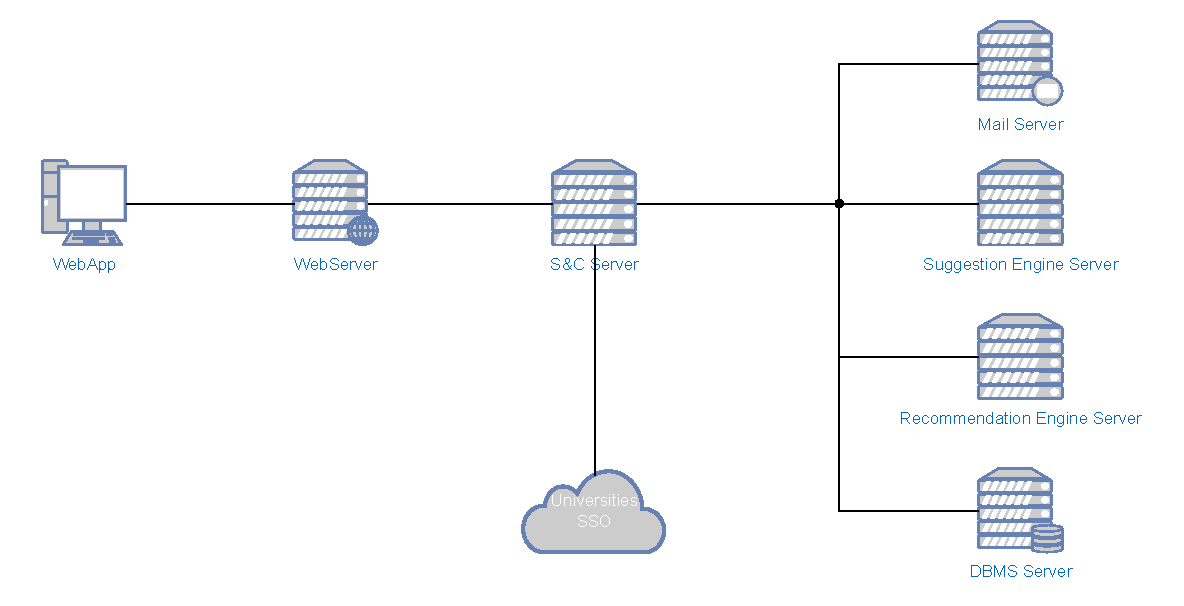
\includegraphics[width=1.0\textwidth]{Images/Overview_diagram.pdf}
      \caption{S\&C Architecture Overview}
      \label{fig:overview}
\end{figure}

\par On the client side can be seen:

\begin{itemize}
      \item \textbf{WebApp}: The web application that the user interacts with, allowing users to connect to S\&C.
            It displays the user interface and sends the user's requests to the core server.
\end{itemize}

\par On the server side, we can see:

\begin{itemize}
      \item \textbf{Web Server}: It handles communication between users and the S\&C system. It is responsible for
            serving the user interface and processing user requests by forwarding them to the S\&C Server.
            Additionally, it manages user sessions and contains the necessary configuration for student authentication
            through university Single Sign-On (SSO) services.
      \item \textbf{S\&C Server}: The main server of the S\&C system. It is the core component and is responsible
            for communication between the Web Server and the databases and the APIs/Services.
      \item \textbf{DBMS Server}: This server archives all the essential information of the system.
            It stores data related to Users, CVs, Internship Advertisements, and Complaints.
      \item \textbf{Recommendation Engine Server}: This server is responsible for generating recommended Internship
            Advertisements for students and anonymous CVs for companies.
      \item \textbf{Suggestions Engine Server}: This server is responsible for generating suggestions for improving
            students' CVs and companies' internship advertisements.
      \item \textbf{Mail Server}: This server is responsible for sending emails to users. It is used for sending
            notifications and confirmations of actions performed by users.
\end{itemize}

\section{Component View}
\label{sec:component-view}%

\subsection{High-Level Components}
\label{sub:high-level-components}%

\begin{figure}[H]
      \centering
      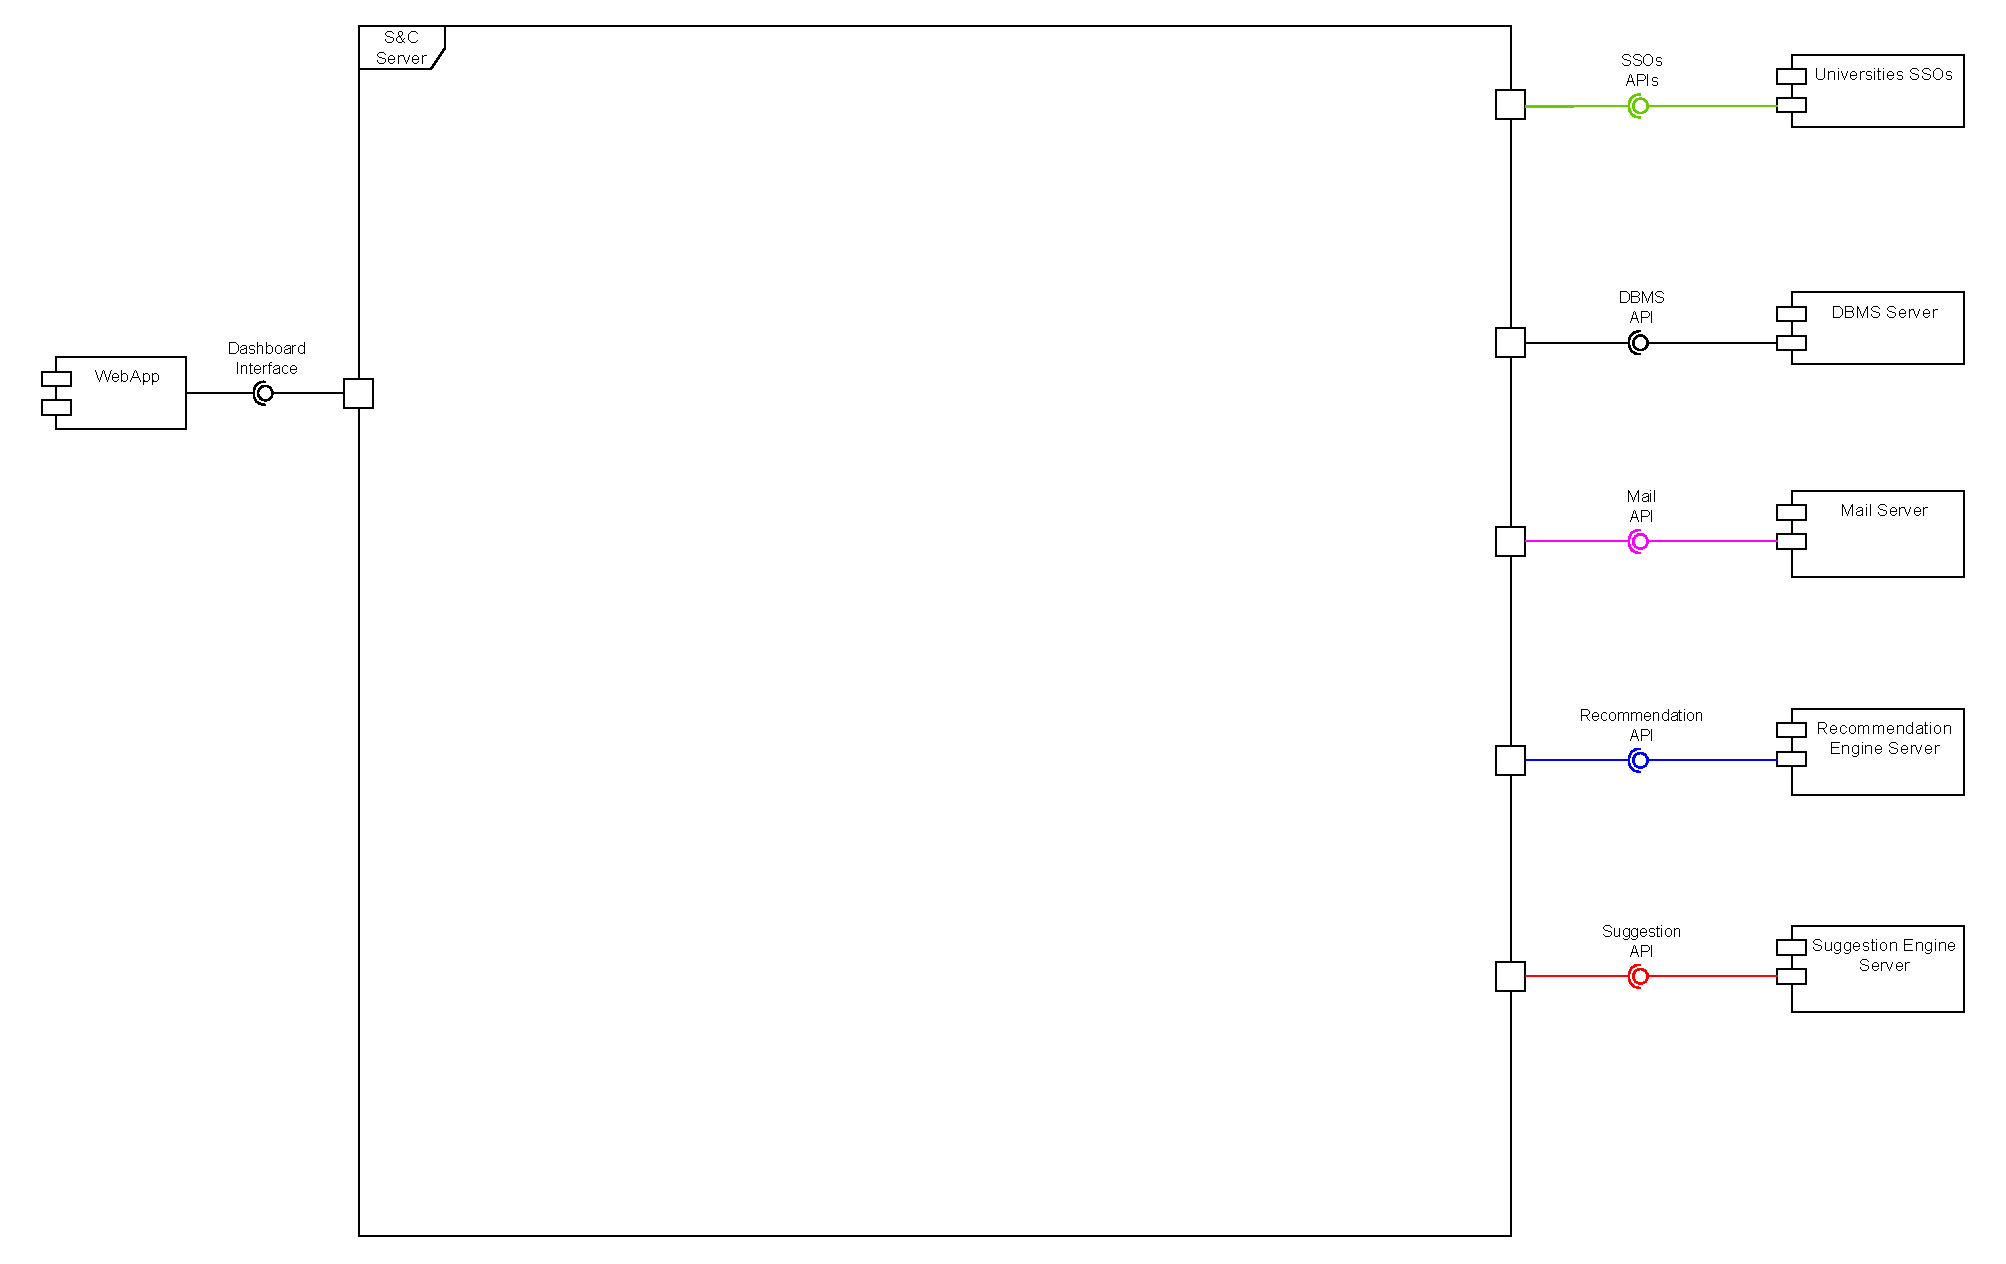
\includegraphics[width=0.8\textwidth]{Images/High_Level_Architectural_Design.pdf}
      \caption{High-Level Components}
      \label{fig:high-level-components}
\end{figure}

\par Figure \ref{fig:high-level-components} shows the high-level components of the S\&C system. The main external components are:

\begin{itemize}
      \item \textbf{WebApp}: This is the web application that the user interacts with. It allows users to communicate
            with the S\&C Server through the Dashboard Interface, which is the only means of interaction
            between the users and the system. The Dashboard Interface includes multiple functionalities,
            one of which allows the Dashboard to send notifications to users while they are using the system.
      \item \textbf{DBMS Server}: This server stores all the information of the Users, including their profile information, CVs,
            Internship Advertisements, Questionnaires, and Complaints. It is the main component of the system and is
            responsible for data management.
      \item \textbf{Mail Server}: This server is responsible for notifying users outside of the web application.
            It is used to send all types of notifications, including those confirming actions performed by a user,
            notifications of new recommendations for both students and companies, requests to fill out questionnaires,
            and notifications about the creation of new complaints, etc.
      \item \textbf{Recommendation Engine Server}: This server is responsible for generating recommended Internship Advertisements for students
            and anonymous CVs for companies. It periodically retrieves CV data and Internship Advertisement data
            to improve the program responsible for creating suggestions for each user.
      \item \textbf{Suggestions Engine Server}: This server is responsible for generating suggestions for improving students' CVs and companies' internship advertisements.
            It periodically retrieves CV data, Internship Advertisement data, and feedback answers at the end of internships
            to improve the program responsible for creating suggestions for each user.
      \item \textbf{Universities SSOs}: This external component allows students to log in to the system using their university credentials.
\end{itemize}

\subsection{Low-Level Components}
\label{sub:low-level-components}%

\begin{figure}[H]
      \centering
      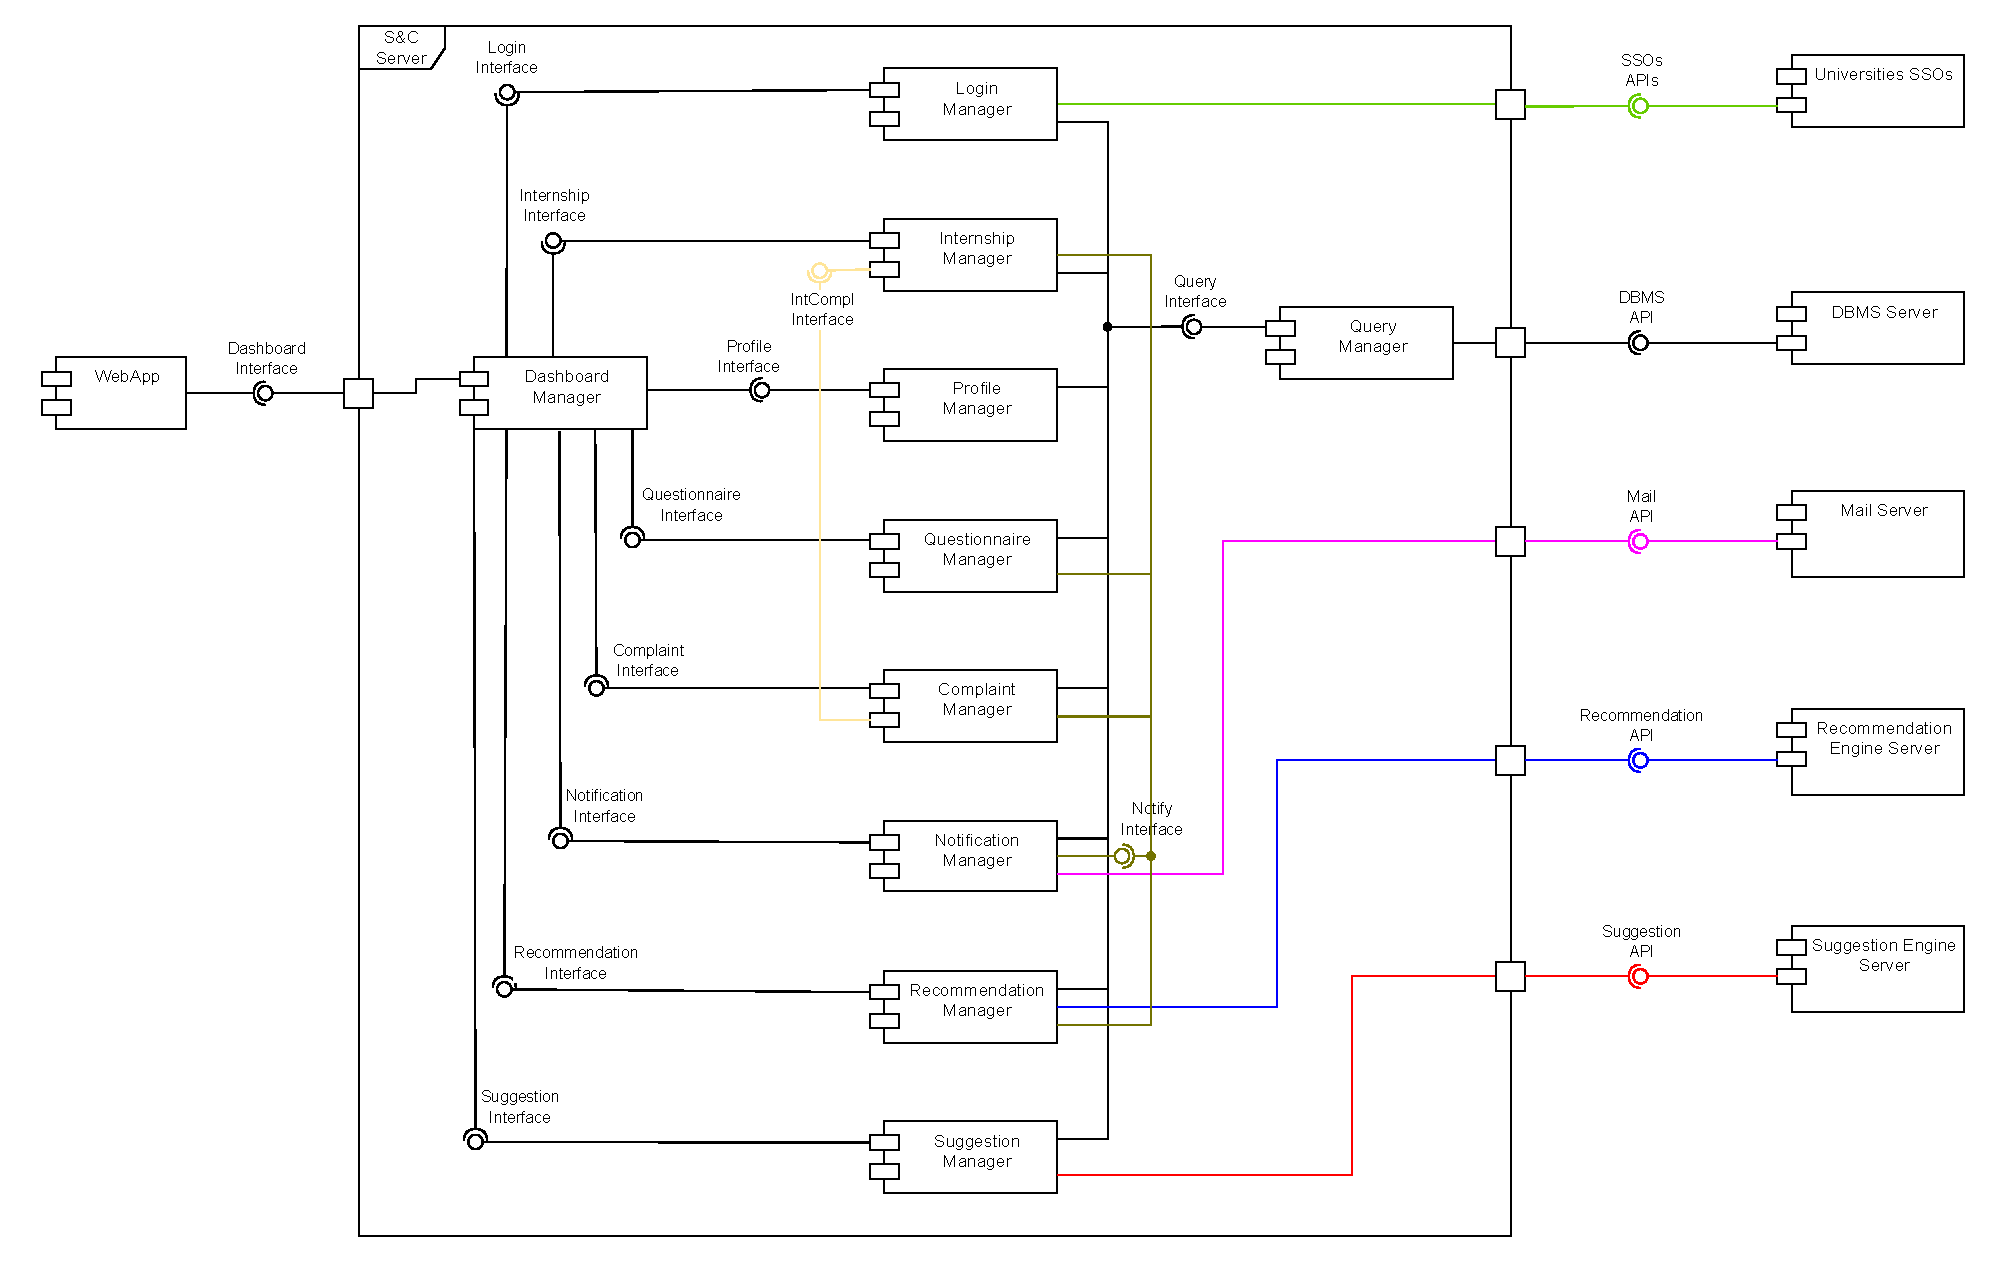
\includegraphics[width=1.0\textwidth]{Images/Low_Level_Architectural_Design.pdf}
      \caption{Low-Level Components}
      \label{fig:low-level-components}
\end{figure}

\par Figure \ref{fig:low-level-components} shows the complete architecture of the S\&C system, detailing the components inside the S\&C Server:

\begin{itemize}
      \item \textbf{Dashboard Manager}: This component is responsible for interacting with users through the dashboard interface.
            The Dashboard Manager executes user requests and interacts with the appropriate components.
      \item \textbf{Login Manager}: This component is responsible for user login. For companies and universities,
            it checks credentials against those stored in the DBMS. For students, it handles the first login (registration)
            and subsequent logins by interacting with the Universities SSOs.
      \item \textbf{Internship Manager}: This component manages all stages of the Internship selection and execution process.
            It handles the creation of Internship Advertisements, the list of student applications,
            and the status of internships. It also provides an interface for the Complaint Manager to modify the status of internships.
      \item \textbf{Profile Manager}: This component manages user profiles. It allows users to modify their profile information,
            students to upload their CVs, and companies to create their profile descriptions.
      \item \textbf{Questionnaire Manager}: This component manages Questionnaires, both those created by companies for selecting students for internships
            and those created by the system for feedback at the end of internships.
      \item \textbf{Complaints Manager}: This component manages complaints. It is used to create complaints, manage them, and if necessary,
            interact with the related internship to modify its status through the interface provided by the Internship Manager.
      \item \textbf{Notification Manager}: This component manages notifications. It generates notifications to send to the
            dashboard if the user is logged in, and interacts with the Mail Server to send notifications to users outside of the web application.
      \item \textbf{Recommendation Manager}: This component interacts with the Recommendation Engine Server. It retrieves the data
            required by the recommendation engine to improve its suggestions, and retrieves the results of the recommendation engine to display to users.
      \item \textbf{Suggestions Manager}: This component interacts with the Suggestions Engine Server. It retrieves the data
            required by the suggestion engine to improve its suggestions, and retrieves the results of the suggestion engine to display to users.
      \item \textbf{Query Manager}: This component executes queries and converts the data returned by the DBMS into the necessary objects for other components.
\end{itemize}

\subsubsection{Login Manager}
\label{subsub:login-manager}%

\begin{figure}[H]
      \centering
      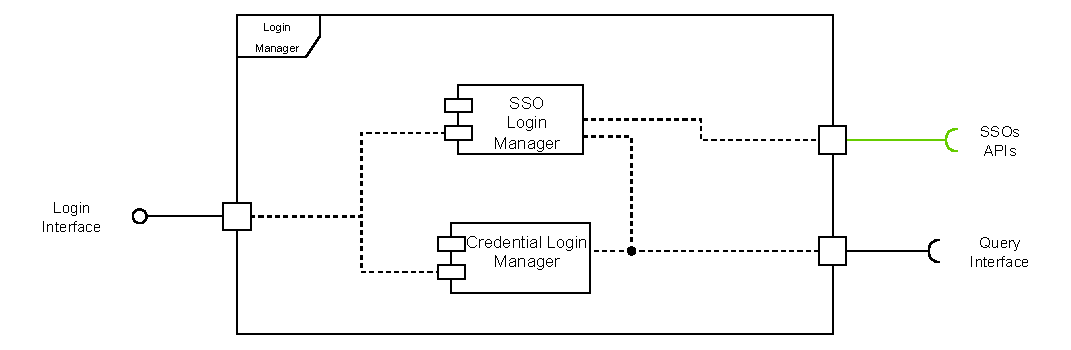
\includegraphics[width=0.8\textwidth]{Images/Login_Architecture.pdf}
      \caption{Login Manager}
      \label{login-manager-arch}
\end{figure}

\par The Login Manager is composed of other two sub-components:
\begin{itemize}
      \item \textbf{Student Login Manager}: This component is responsible for managing student logins
            and their registration. It interacts with the Universities SSOs to authenticate students.
      \item \textbf{COUN Login Manager}: This component is responsible for managing company and university logins.
            It checks the credentials against those stored in the DBMS.
\end{itemize}

\subsubsection{Internship Manager}
\label{subsub:internship-manager}%

\begin{figure}[H]
      \centering
      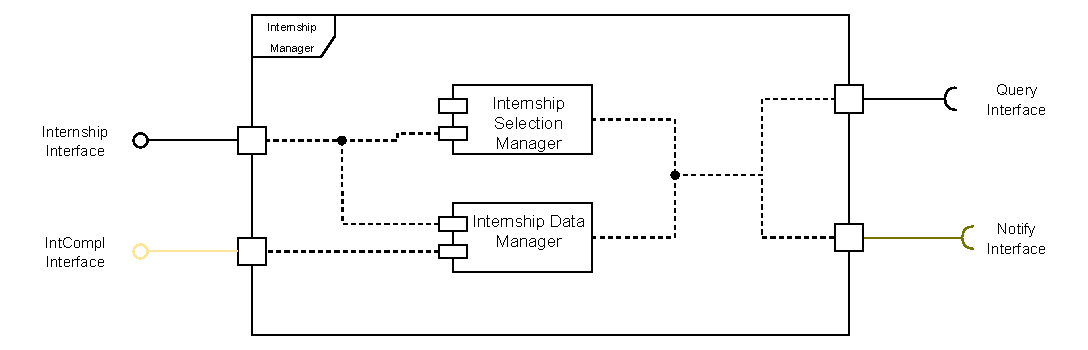
\includegraphics[width=0.8\textwidth]{Images/Internship_Architecture.pdf}
      \caption{Internship Manager}
      \label{internship-manager-arch}
\end{figure}

\par The Internship Manager is composed of other two sub-components:
\begin{itemize}
      \item \textbf{Internship Selection Manager}: This component is responsible all the stages of the internship selection process.
            It handles the creation of internship advertisements, the list of student applications.
      \item \textbf{Internship Data Manager}: This component is responsible for managing the status of internships,
            who's the responsible for the internship, the descriptions of it, the requirements and the duration.
            It also provides an interface for the Complaint Manager to modify the status of internships.
\end{itemize}

\subsubsection{Profile Manager}
\label{subsub:profile-manager}%

\begin{figure}[H]
      \centering
      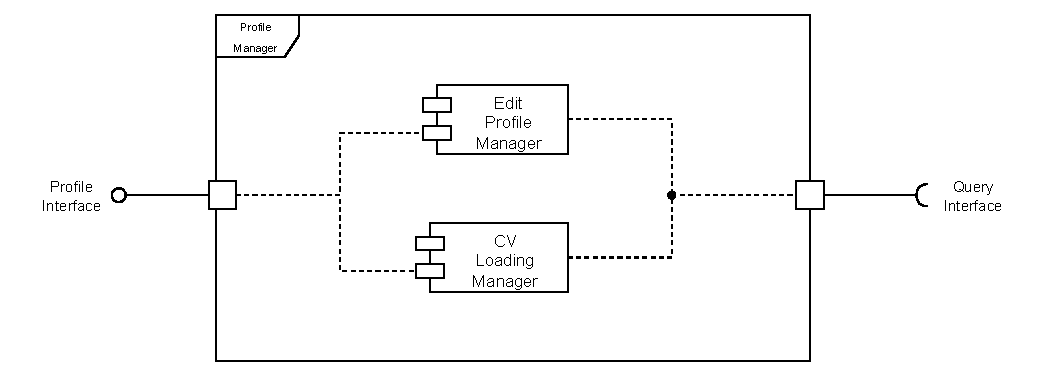
\includegraphics[width=0.8\textwidth]{Images/Profile_Architecture.pdf}
      \caption{Profile Manager}
      \label{profile-manager-arch}
\end{figure}

\par The Profile Manager is composed of other two sub-components:
\begin{itemize}
      \item \textbf{Profile Manager}: This component is responsible for the modification of the user's profile information.
            For the companies it allows to create their profile description that will be shown to students.
      \item \textbf{CV Manager}: This component is responsible for the management of the student's CVs and uploading them.
\end{itemize}

\subsubsection{Questionnaire Manager}
\label{subsub:questionnaire-manager}%

\begin{figure}[H]
      \centering
      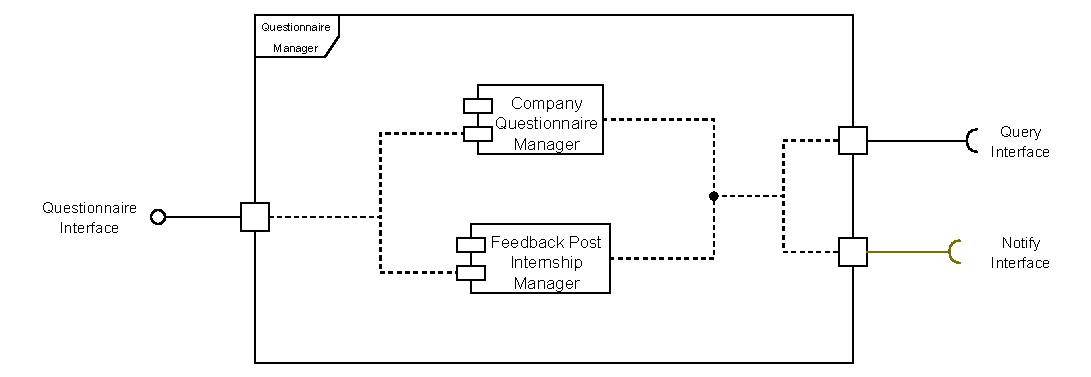
\includegraphics[width=0.8\textwidth]{Images/Questionnaire_Architecture.pdf}
      \caption{Questionnaire Manager}
      \label{questionnaire-manager-arch}
\end{figure}

\par The Questionnaire Manager is composed of other two sub-components:
\begin{itemize}
      \item \textbf{Company Questionnaire Manager}: This component is responsible for managing the questionnaires created by companies.
            It allows companies to create, modify and delete questionnaires to select students for internships.
            It allows companies to see the answers to the questionnaires.
      \item \textbf{Feedback Questionnaire Manager}: This component is responsible for managing the feedback questionnaires created by the system.
            It allows the system to create questionnaires for feedback at the end of internships.
\end{itemize}

\section{Deployment View}
\label{sec:deployment-view}

\begin{figure}[H]
      \centering
      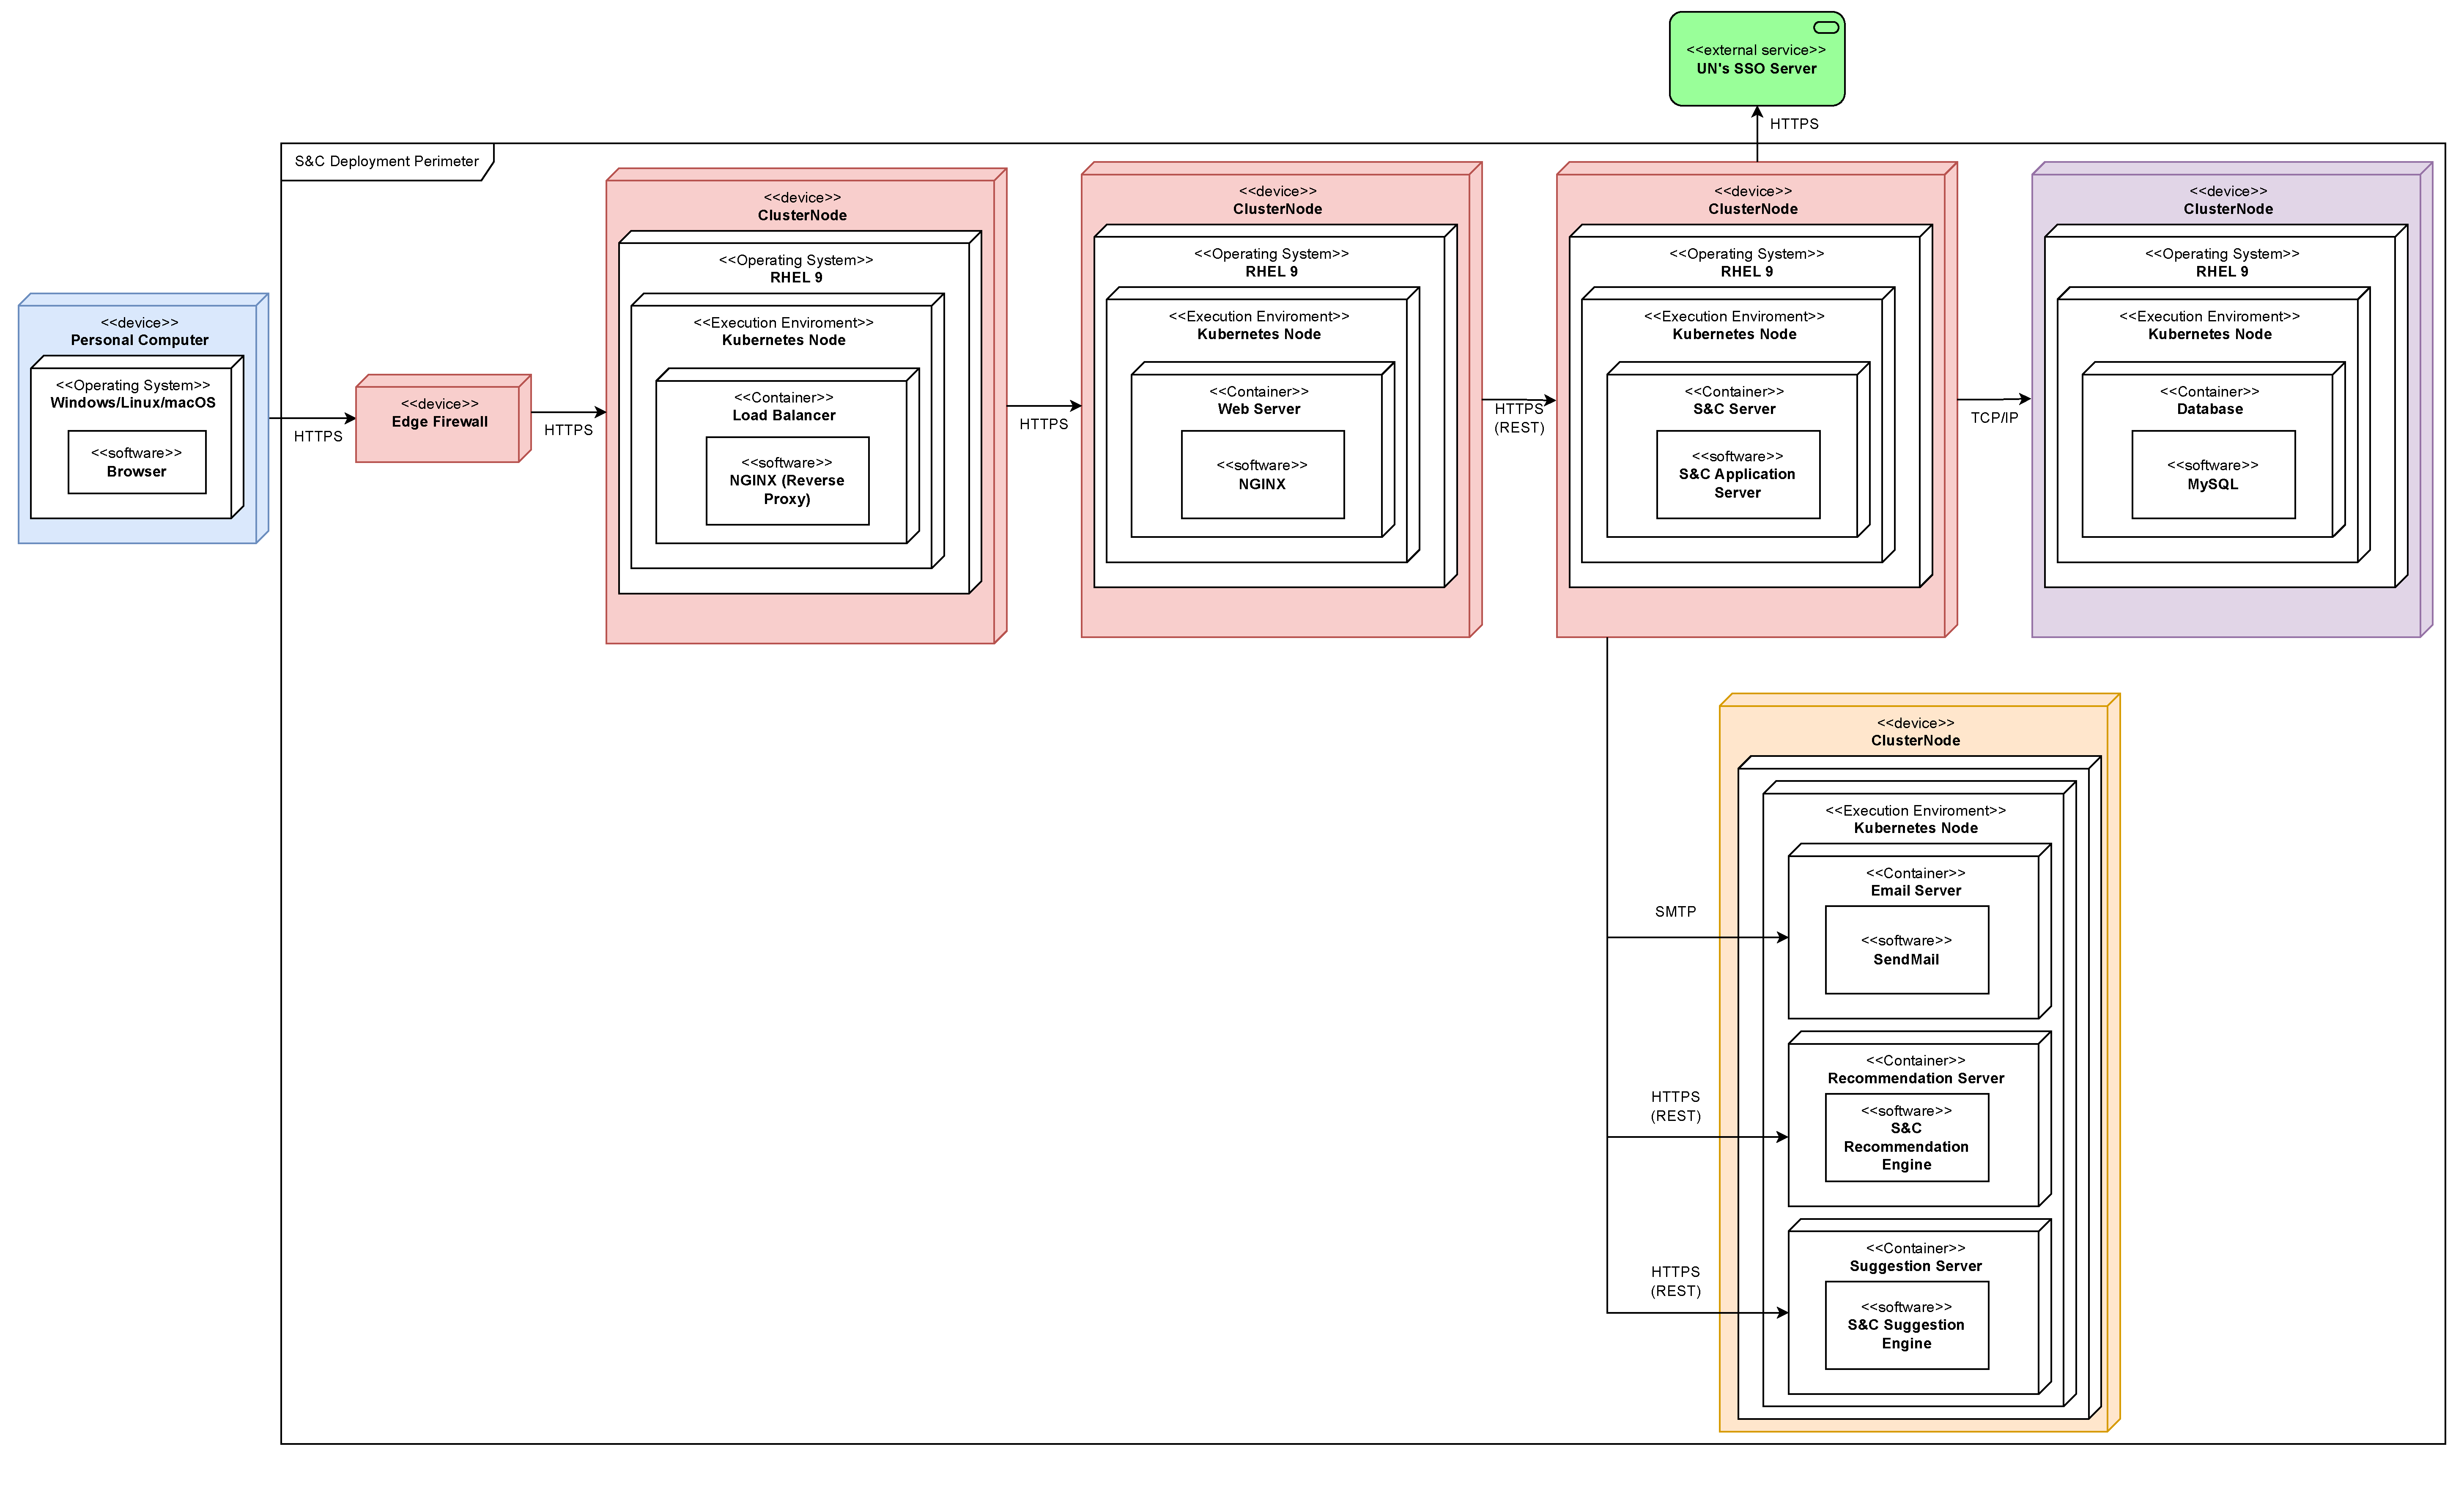
\includegraphics[width=1.0\textwidth]{Images/Deployment_Diagram.pdf}
      \caption{Deployment Diagram}
      \label{fig:deployment-diagram}
\end{figure}

% This should be section 2.6. of the DD.

\section{Selected Architectural Styles and Patterns}
\label{sec:selected-architectural-styles-patterns}%

\par{\textbf{Architectural Design:}} The architectural design of S\&C is based on the industry-standard 3-Tier-Architecture pattern:

\begin{enumerate}
      \item \textbf{Presentation Tier:} This is the upper layer that directly interacts with users. The presentation tier
            focuses on displaying information to the user and capturing user inputs. It's designed to handle all client-side
            interactions and renders the application's visual components.
      \item \textbf{Application Tier:} This layer contains the core business logic and processing rules of the
            application. It receives requests from the presentation tier, applies business rules, validates data, and
            coordinates the flow of information. This tier acts as an intermediary, ensuring that data is processed
            according to the application's specific requirements before being passed to or retrieved from the data tier.
      \item \textbf{Data Tier:} The bottom layer of the architecture, responsible for storing, retrieving, and managing
            data. The data tier ensures data integrity, provides database connection management, and implements data
            access methods that the application tier can use to interact with the stored information.
\end{enumerate}

The division of the system into these three layers allows a reduction in complexity, improves maintainability, and
facilitates scalability: each layer can be developed, tested, deployed and maintained independently, enabling a more
modular and flexible system architecture while also paralleling development efforts.

The choice of a 3-Tier-Architecture is also motivated by the fact that it can be easily mapped to the MVC
(Model-View-Controller) pattern - a widely-used design pattern that separates the application into three interconnected
components: the Model (data), the View (interface), and the Controller (business logic). This pattern is particularly
useful since it allows for a clear separation of concerns and a more modular and maintainable codebase.

Each tier will be run inside a container environment (e.g. Docker) to ensure isolation and scalability. The containers
will be orchestrated (using adequate solutions e.g. Kubernetes) which will also manage the deployment and scaling of
the application.

\par{\textbf{Client-Server Communication:}} S\&C - like almost all modern web applications - is based on a
Client-Server architecture. The client (the user's browser) sends requests to the server, which processes them and
returns the appropriate responses. All the static content (HTML, CSS, JavaScript) is served directly using HTTPS, while
the dynamic content is generated by the server and sent back to the client as JSON data (REST over HTTPS) to be
rendered by the client-side JavaScript code.

\par{\textbf{Intra-Server Communication:}} The communication between the presentation tier and the application tier
will be based on gRPC over TCP/IP. gRPC is a high-performance, open-source, universal RPC framework that can run in any
environment allowing for an easy and efficient communication between the two tiers. The communication between the
application tier and the data tier will be based on SQL Queries over TCP/IP (as implemented by the database driver).

\section{Other Design Decisions}
\label{sec:other-design-decisions}%

\par{Helpers:} In \ref{sec:selected-architectural-styles-patterns} we said that the application tier is running inside a
container. While this is true it must be noted that the application is not fully monolithic. The application tier is
composed of:

\begin{itemize}
      \item \textbf{Core:} The core of the application, it contains the business logic and the processing rules. It is
            the part that communicates with the data tier and the presentation tier.
      \item \textbf{Email Service:} A service that sends emails to users. It is a separate service because it is not
            strictly related to the core of the application and it can be easily scaled independently. Communicates
            with the core using SMTP over TCP/IP. Core prepares the email and sends it to the email service which
            sends it to the user.
      \item \textbf{Recommendation Engine:} A service that provides internships recommendations to STs. Communicates
            with the core using gRPC over TCP/IP. Core asks the recommendation engine for recommendations and the
            recommendation engine provides them.
      \item \textbf{Suggestion Engine:} A service that proposes STs to COs (as described in the RASD). Communicates with
            the core using gRPC over TCP/IP like the recommendation engine.
\end{itemize}

It should be also remarked that the application tier communicates with (external to S\&C) the various UN's SSOs using
HTTPS.

\par{\textbf{Networking:}} The internal S\&C network will solely rely on IPv6. This choice is motivated by the fact that
IPv6 is cheaper to maintain, more secure, and more scalable than IPv4. The load balancer at the edge will provide IPv4
connectivity to the outside world for compatibility reasons but all internal communication will be done using IPv6.
This choice will also make easier a multi-cloud deployment in the future.
